%!TEX root = main.tex
% UTF-8 encoding
\section{Discussion}
\label{sec:dis}
Our algorithms rely on a small number of hyper-parameters and choices of classification models. 
In this  section, we demonstrate how to choose these hyper-parameters through detailed ablation studies, primarily on  the drug dataset.
% The discussion primarily relies on the drug dataset, owing to the fact 
% that drug-related euphemisms are numerous and evolve very rapidly. 

\subsection{Ablation Studies for Euphemism Identification}
As discussed above, we adopt a coarse-to-fine-grained classification scheme for euphemism identification, relying on two classifiers used in cascade. 
We discuss here the performance of multiple classifiers on both coarse and fine-grained classification. 

\subsubsection{Coarse Classifiers}
\label{sec:ablation_coarse}
\begin{figure}[ht!]
	\centering
	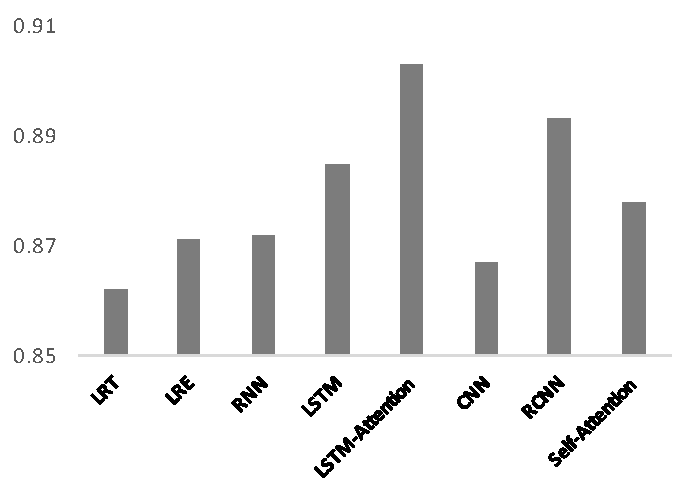
\includegraphics[width=0.7\linewidth]{figures/11}
	\caption{Testing accuracy for the coarse classifier.}
	\label{fig:11}
\end{figure}

In the euphemism identification framework, we use a binary classifier to filter out the sentences where euphemisms are used in non-euphemistic senses. 
We experiment with the binary classifiers shown below. Note that for all the neural models, we use 100-dimensional GloVe embeddings \cite{pennington2014glove} pre-trained on Wikipedia\footnote{\url{https://nlp.stanford.edu/projects/glove/}} and tune the embeddings by the models. 
\begin{itemize}
	\item Logistic Regression \cite{hosmer2013applied} on raw text (LRT): we first represent each word as a one-hot vector and then represente each sentence as the average of its member words' encodings. 
	\item Logistic Regression on text embeddings (LTE): we learn the word embeddings (100-dimensional) using word2vec \cite{mikolov2013distributed,mikolov2013efficient}. 
	We represent each sentence by the average of its member words' embeddings. 
	\item Recurrent Neural Network (RNN) \cite{rumelhart1985learning}: we use a 1-layer bidirectional RNN with 256 hidden nodes. 
	\item Long Short-Term Memory (LSTM) \cite{hochreiter1997long}: we use a 1-layer bidirectional LSTM with 256 hidden nodes. 
	\item LSTM-Attention: we add an attention mechanism \cite{bahdanau2015neural} on LSTM. 
	%The attention model computs soft alignment scores between each of the hidden_state and the last hidden_state of the LSTM.
	\item Convolutional Neural Networks (CNN) \cite{kim2014convolutional}: we train a simple CNN with one layer of convolution on top of word embeddings. 
	\item Recurrent Convolutional Neural Networks (RCNN) \cite{lai2015recurrent}: we apply a bidirectional LSTM and employ a max-pooling layer across all sequences of texts. 
	\item Self-Attention \cite{lin2017structured}: Instead of using a vector, we use a 2-D matrix to represent the embedding, with each row of the matrix attending on a different part of the sentence. 
\end{itemize}


We split the datasets into 70-10-20 for training, validation and testing. 
The model parameters are tuned on the validation data. 
Empirically, we find the LSTM-Attention performs the best across three datasets. This is  why we ultimately selected it and reported results using it in Section~\ref{sec:res}. 
Yet, as shown in Figure \ref{fig:11}, other classifiers have satisfactory performance as well, and reach a testing accuracy ranging from 0.86 to 0.90. 

\subsubsection{Fine-Grained Classifiers}
\label{sec:ablation_fine-grained}
In the euphemism identification framework, we use a multi-class classifier to identify to which target keyword each euphemism refers. 
Again, we experimented with the same set of classifiers as above.
Interestingly, we find that, for fine-grained classification, 
all classifiers have highly similar results. 
One possible reason is that each class has relatively small number of training instances (ranging from a few hundreds to 100k), which limits the discriminative power of advanced algorithms. 
For the drug dataset (33 target keywords), the training accuracy is about 55\% and the testing accuracy is about 24\%. 
This shows the feasibility of the task since the random guess accuracy would be 3.3\%. 
Given the similar performance across  classifiers, we recommend  Logistic Regression on raw text for better computational efficiency. 



\subsection{Parameter Analysis}
\label{sec:dis_parameter_analysis}
\begin{figure}[ht!]
	\centering
	\vspace{-0.5cm}
	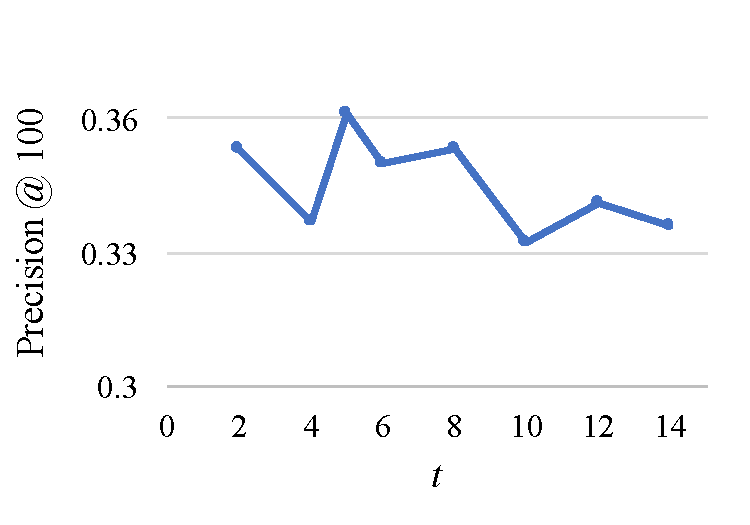
\includegraphics[width=0.7\linewidth]{figures/12}
	\caption{Sensitivity of $t$.}
	\label{fig:12}
\end{figure}

In the euphemism detection step 
(Section \ref{sec:model_det}), 
we set a masked language model threshold~$t$ to filter out the generic masked sentences. 
In the ranked list of replacements for the mask token, if any target keyword appears in the top-$t$ 
replacement candidates for the masked sentence, 
we consider  the masked sentence a valid context instance. % for the context of interest. 
Otherwise, we considere  the masked sentence generic and filter it out. 
Figure \ref{fig:12} shows how the results change with the threshold $t$ and we observe a slight decrease when the threshold $t$ is larger than 5. So, $t=5$ appears to be an optimal parameter choice.


\subsection{Limitations} 
While our approach for euphemism detection and identification
appears highly promising,
it does have some limitations.

\medskip 
\noindent{\textbf{Text-only moderation}}: 
Our approach only works with text, and our techniques
are not easily generalizable to other media.
Social media posts frequently include images, video, and audio,
which can be even more challenging (and even more traumatic)
to moderate by hand~\cite{newton2019terror, newton2019trauma, ofcom:ai2019}.
However, text is frequently associated with these other media, 
\eg, in the form of comments, and thus detecting euphemism use might 
indirectly provide clues to content moderators dealing with 
different media. 

\medskip
\noindent{\textbf{Other contexts}}:
Our approach performs well
on corpora discussing drugs, weapons, and sexuality.
In preliminary experiments
with a corpus of hate speech
it did not perform nearly as well,
producing many false matches
when tasked with identifying racial slurs.
We believe this is because
euphemisms related to drugs, weapons, and sex
typically have specific meanings;
\eg, ``pot'' always refers to marijuana, not some other drug.
Racial slurs, on the other hand,
are (in this corpus)
used imprecisely, and interchangeably with generic swearwords,
which seems to confuse euphemism identification.
We do not know yet whether this is a fundamental limitation.
Even if it is, though,
there are many  contexts where euphemisms have specific meanings
and our approach should be effective,  particularly forums selling illicit goods.
% :
% we are, for instance, planning to test it
% on a corpus of posts from ``darknet'' forums
% discussing credit card fraud and similar crimes.

\medskip
\noindent{\textbf{Robustness to adversarial evasion}}: 
In our evaluation, we have relied on \textit{a priori} 
non-adversarial datasets, 
that were gleaned from public, online forums. 
In other words, people were using euphemisms, 
but we do not know whether they were using them
specifically to evade content moderation.
Perhaps these euphemisms are, for them,
simply the ordinary names of certain things
within the circle where they were discussing them.
(Someone who consistently spoke of ``marijuana'' instead of ``pot''
on a forum dedicated to discussing drug experiences
might well be suspected of being an undercover cop.)

Because our algorithms rely on sentence-level context
to detect and identify euphemisms,
an adversary would need to change that context
to escape detection.
Such changes 
may also render the text unintelligible
to its intended audience.
Therefore, we expect our techniques
to be moderately resilient to adversarial evasion.
However, we cannot test our expectations at the moment,
since we do not have a dataset
where people were purposely using euphemisms
\emph{only} to escape detection.

\medskip
\noindent{\textbf{Usability for content moderators}}:
While our approach shows encouraging performance in lab tests,
we have not yet evaluated
whether it is good enough to be helpful to content moderators in practice.
That evaluation would require a user study of professional content moderators.
This is out of scope for the present paper,
which  focuses on the technical underpinnings
of euphemism detection and identification.
We are interested in investigating usability as a follow-up study.

% Detection Challenges
% Identification Challenges




%\subsection{Limitation and Future Work}
%%We run our experiments on two other datasets with relatively negative results. 
%Euphemistic phrase detection. 




%\subsection{The Effect of Fine-tuning the BERT Model}
%\begin{figure}[ht!]
%	\centering
%	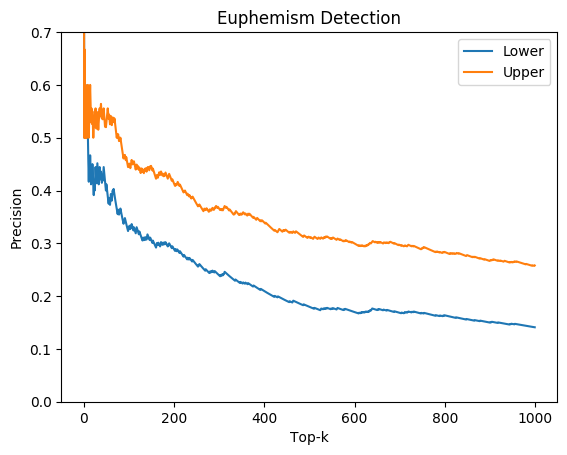
\includegraphics[width=0.48\linewidth]{figures/Precision_reddit}
%	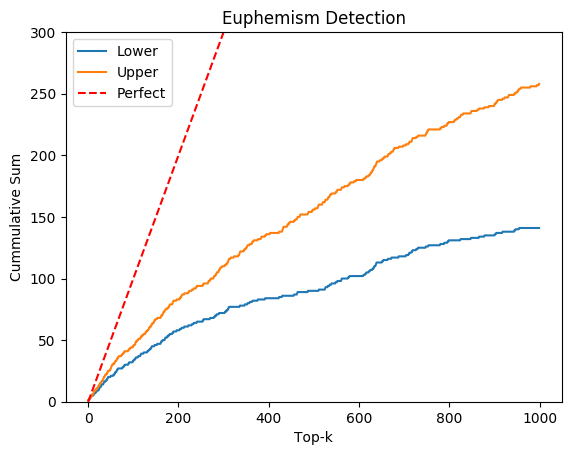
\includegraphics[width=0.48\linewidth]{figures/CSum_reddit}
%	\caption{Left shows the top-k precision \textit{vs.} k on the drug dataset. Right shows the cumulative correct numbers \textit{vs.} k on the drug dataset. }
%	\label{fig:precisionreddit}
%\end{figure}
%We have shown the numeric results of euphemism detection in Table \ref{table:res_dec}. Besides, we show the plots on top-k precision and cummulative correct detections against k in Figure \ref{fig:precisionreddit}. 



%\subsection{Computational Efficiency}
%We did not measure the baselines so far. 
%We implemented all models in Python 3.7 and conducted all the experiments on a computer with twenty 2.9 GHz Intel Core i7 CPUs and one GeForce GTX 1080 Ti GPU. 
%The BERT fine-tuning on the text corpus step took 5.4 hours (3 epochs).
%The euphemism detection took 1.5 hours. 
%The euphemism identification took 1.5 hours. 

